\label{ride-sharing}
\subsubsection{Purpose}

Every subscribed passenger shall be able to activate the ride sharing function in the mobile app or in the web interface. When this mode is enabled, the passenger has to provide the system also with a destination for the ride.

The system, before allocating a taxi, inserts the pending ride in the set of shared rides and tries to identify possible sharing solutions.
With an adeguate algorithm it can propose every feasible sharing solution to the user.

The first user who reserves a taxi is called the ``owner'' of the ride.
The passenger can choose to join one of the pending rides or to refuse the proposal, becoming the owner of a new ride.

In the first case the system informs the owner of the ride. The new passenger has to go to the meeting point with the owner of the ride in time. If he/she is not able to do that the taxi does not wait for him/her.

In the second case the system allocates the taxi (\ref{taxi-availability}) and applies the standard procedure \ref{standard-call}.  The user becomes the owner of the ride.
If there is another user who wants to share the ride with compatible options, the system allows it and redirects this last user to the meeting point with the owner who is informed same as the taxi driver.

\subsubsection{Scenario 1}
Batman needs a taxi and decides to enable the sharing mode on his cell phone. The app requires also the destination point of Batman's travel.

When Batman submits the form, the system matches the path of Batman's ride with every pending ride started from Batman's area. It finds only one compatible ride and sends it to Batman.

Batman finds that it is Joker's pending ride and decides to refuse the share. Then the system allocates a new taxi.

A new user, Robin, is in Batman's area and wants to take a taxi. He decides to enable the sharing function and the system proposes him Batman's and Joker's ones. He chooses Batman's: the system, which has already communicated location and time to Robin, notifies Batman and the taxi driver that there is an additional passenger.

When the taxi arrives, the taxi driver confirms from his mobile app how many passengers he has picked up.

\subsubsection{Use case}
The use case for a ride sharing is shown in~\autoref{usecase-ridesharing}.

\begin{table}
\begin{center}
\begin{tabular}{| l | p{0.6\textwidth} |}
\hline
Actor & Taxi driver and Multiple Passengers \\
\hline
Goal & Goal~\ref{g-share}
\\
\hline
Input condition & The user enables the sharing option from his mobile phone or from the web interface.  \\
\hline
Event Flow & \begin{enumerate}
	\item The user enables the sharing option
	\item The user must enter a destionation
	\item The system computes the possible sharing rides and proposes them to the user.
	\item The user can accept a sharing option or refuse all of them
	\item If the user refuses the system executes the standard taxi call \ref{standard-call}, otherwise notifies the owner of the ride and the taxi driver
	\end{enumerate}
\\
\hline
Output condition & The system informs the owner of the ride and the taxi driver that the ride will be shared. \\
\hline
Exception & No taxi available in the area. \\
\hline
\end{tabular}
\end{center}
\caption{Use case for ride sharing.}
\label{usecase-ridesharing}
\end{table}

\subsubsection{Response sequence}
The response sequence is illustrated in figure \ref{fig:sequence-sharing}

\begin{figure}
	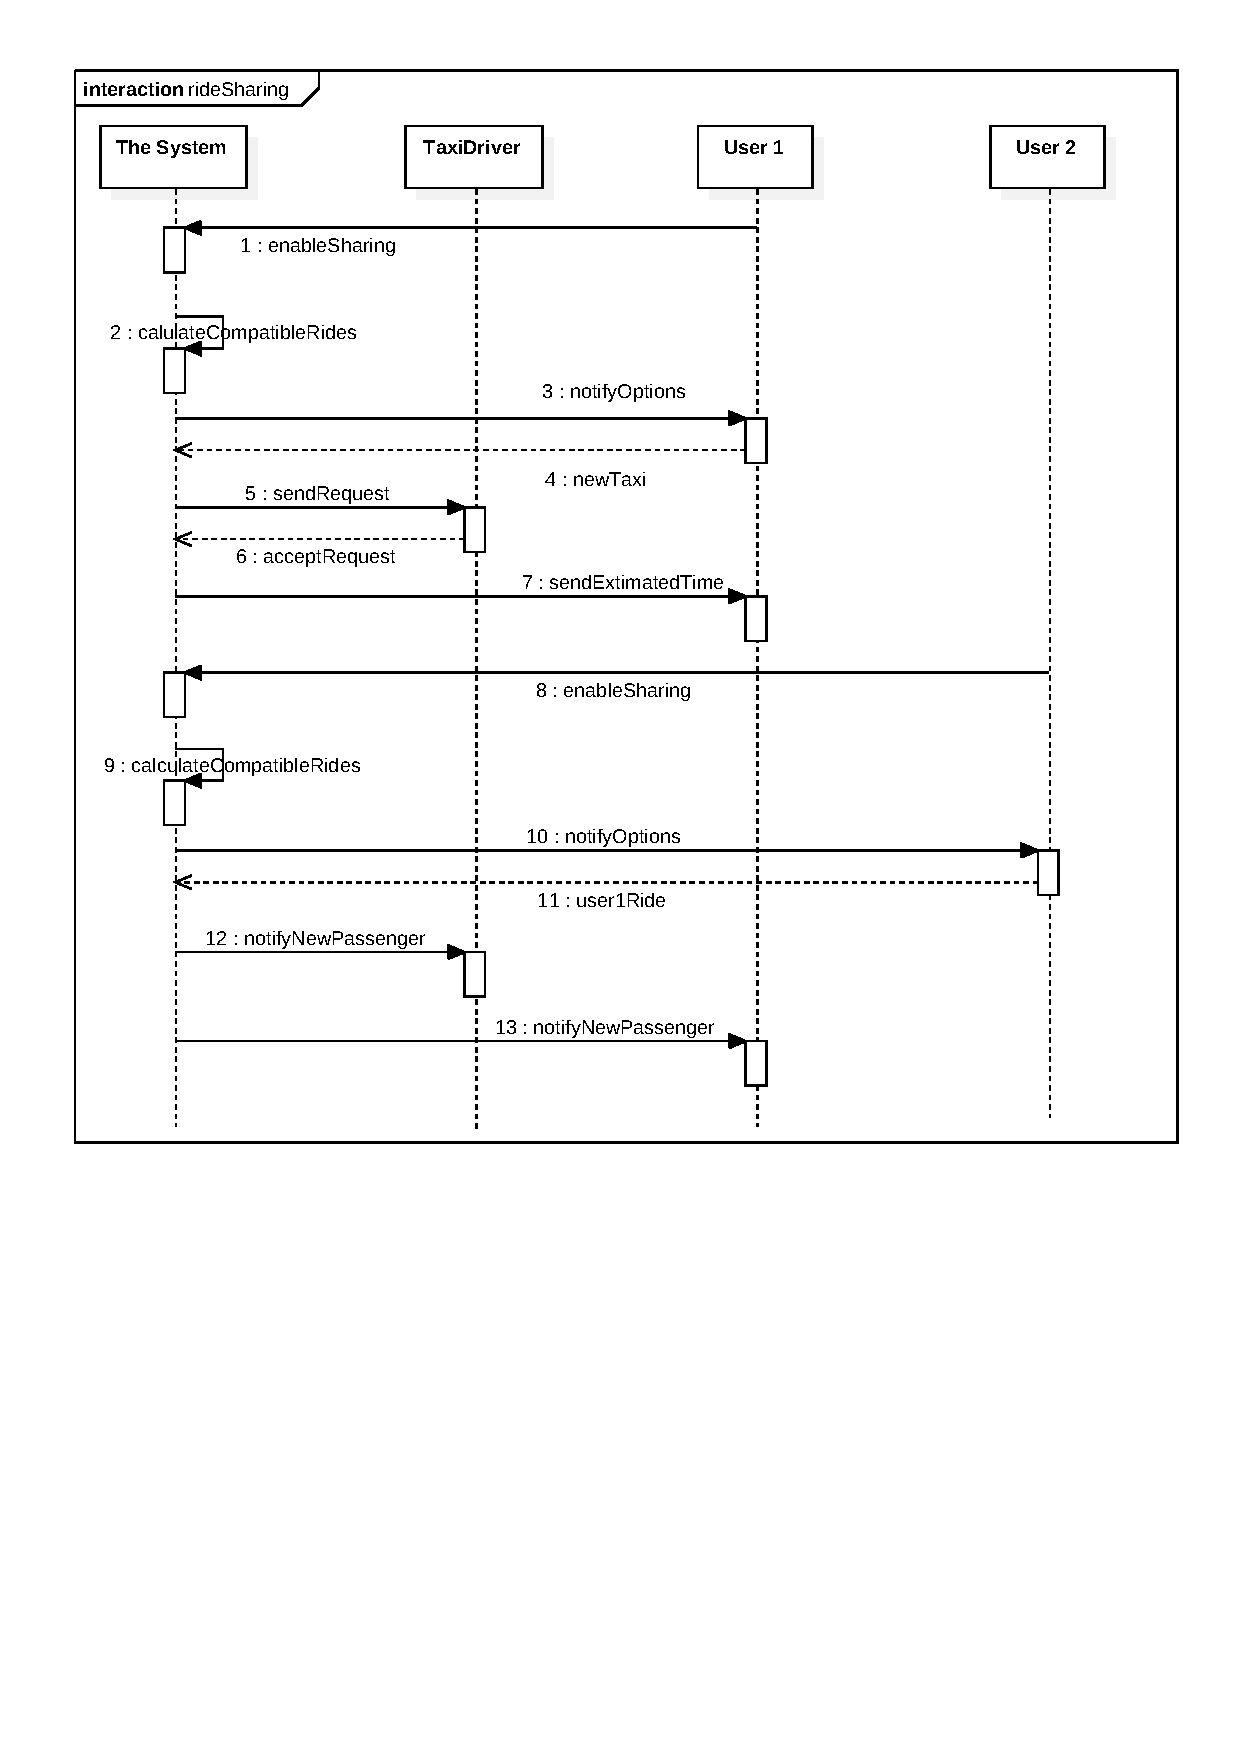
\includegraphics[width=\textwidth]{diagrams/ride_sharing.pdf}
	\caption{Sequence diagram of a ride sharing.}
	\label{fig:sequence-sharing}
\end{figure}

\subsubsection{Associated functional requirements}
\begin{enumerate}
\item The system has to know the starting point of the new passenger in order to provide physical sharing solutions. It has to compute the estimated walking time to reach the meeting location and compare it with the estimated taxi arrival time.
\item The user can enable the sharing function both in mobile app and in web interface.
\item The user can choose between possible sharing solutions or a new taxi.
\item The system has to communicate to the taxi driver the possible presence of the new passenger.
\item The system must be able to analyse the current sharing situation.
\item The system must evaluate the number of seats available in every taxi.
\item The taxi driver can insert the number of passengers who have been picked up.
\item After the user chooses to enable the sharing mode, the system has to specify, for every sharing ride, the location and the time.
\end{enumerate}
